%% ==============================================================
%% WARNING! ENGLISH SPEAKING AUTHORS SHOULD READ gretsien.tex
%%          FILE INSTEAD
%% ==============================================================
%% EXEMPLE DE CONTRIBUTION AU GRETSI
%% POUR LES UTILISATEURS FRANCOPHONES DE LaTeX2e
\documentclass{gretsi}
%% Selectionnez ensuite les paquets que vous utilisez,
%% par suppression ou adjonction d'un caractere %
%% en debut de ligne (mise en commentaire).
%% --------------------------------------------------------------
%% UTILISATION DE CARACTERES ACCENTUES AU CLAVIER ?
%% (le codage du clavier depend du systeme d'exploitation)
% \usepackage[applemac]{inputenc} % MacOS
% \usepackage[ansinew]{inputenc}  % Windows ANSI
% \usepackage[cp437]{inputenc}    % DOS, page de code 437
% \usepackage[cp850]{inputenc}    % DOS, page de code 850
% \usepackage[cp852]{inputenc}    % DOS, page de code 852
% \usepackage[cp865]{inputenc}    % DOS, page de code 865
% \usepackage[latin1]{inputenc}   % UNIX, codage ISO 8859-1
% \usepackage[decmulti]{inputenc} % VMS
% \usepackage[next]{inputenc}
% \usepackage[latin2]{inputenc}
% \usepackage[latin3]{inputenc}
%% --------------------------------------------------------------
%% REGLES DE TYPOGRAPHIE FRANCAISES ?
% \usepackage[style=ieee, backend=biber, minnames=1, maxnames=3, url=false]{biblatex}
\usepackage{graphicx}
\usepackage[english,french]{babel}   % "babel.sty" + "french.sty"
\usepackage{times}			% ajout times le 30 mai 2003
 
%% --------------------------------------------------------------
%% CODAGE DE POLICES ?
%% Si votre moteur Latex est francise, il est conseille
%% d'utiliser le codage de police T1 pour faciliter la césure,
%% si vous disposez de ces polices (DC/EC)
\usepackage[utf8]{inputenc}
\usepackage[T1]{fontenc}
\usepackage[single=true, macros=true, xspace=true]{acro}
\usepackage{cleveref}

%% Acronym definition example using glossaries package
%% \usepackage{acro} is required
%% 
%% For a powerful usage of the acro package look at http://tex.stackexchange.com/questions/135975/how-to-define-an-acronym-by-using-other-acronym-and-print-the-abbreviations-toge

\DeclareAcronym{rnc}{
  short = RNC,
  long = Réseau Neuronal Convolutif
}

\DeclareAcronym{pca}{
  short = ACP,
  long = Analyse en Composantes Principales
}

\DeclareAcronym{mcr}{
  short = MCR,
  long = Microscopie Confocale par Réflectance
}

\DeclareAcronym{svm}{
  short = SVM,
  long = Support Vector Machine
}

 
% \bibliography{content/bibliography.bib}
\bibliographystyle{custom_unsrt}

%% ==============================================================

\titre{Extraction et évaluation de caractéristiques adaptées pour la classification du Lentigo à partir d'images de Microscopie Confocale}

\author{\coord{Romain}{Cendre}{1},
        \coord{Alamin}{Mansouri}{1},
        \coord{Jean-Luc}{Perrot}{2},
        \coord{Elisa}{Cinotti}{3},
        \coord{Franck}{Marzani}{1}}
    
\address{\affil{1}{Laboratoire ImViA EA 7535, Université de Bourgogne, Dijon, France}
         \affil{2}{Service de Dermatologie-Oncologie-Allergologie, CHU de St Etienne, France}
         \affil{3}{U.O. Dermatologia, Dipartimento di Scienze Mediche, Università degli Studi di Siena, Italie}}

%%%%%%%%%%%%%%%%%%%%%%%%%%%%%%%%%%%%%%%%%%%%%%%%%%%%%%%%%%%%%%%%%%%%%%%%%%%%%%%

\email{romain.cendre@gmail.com,
alamin.mansouri@u-bourgogne.fr, j.luc.perrot@chu-st-etienne.fr,
elisacinotti@gmail.com, franck.marzani@u-bourgogne.fr}

\resumefrancais{La détection de cancer de la peau est l'un des défis de ces dernières décennies. Par ailleurs, diverses techniques d'imagerie ont pour objectif d'aider à la reconnaissance de ces pathologies malignes en contexte clinique. La Microscopie Confocale par Réflectance est un exemple de technique d'imagerie adaptée à la détection de maladie de la peau sur laquelle nous nous basons pour la détection de Lentigo. Les travaux présentés dans cet article portent sur la classification de ces images en trois catégories : sain, bénin et malin. Dans ce but, nous proposons et évaluons deux méthodes d'extraction de caractéristiques basées sur les descripteurs d'Haralick pour l'une et sur une extraction par Réseau Neuronal Convolutif pour l'autre. Ces deux méthodes sont évaluées et comparées à un travail suggérant une approche par ondelettes, étendu à ces même catégories. D'après les résultats obtenus, l'approche par Réseau Neuronal Convolutif est la plus adaptée à cette problématique.}

\resumeanglais{Detection of skin cancer in time used to be a challenge over decades. In clinical circumstances, a couple of imaging techniques aims to improve early recognition of malignant pathologies. For instance, Reflectance Confocal Microscopy modality is a suitable technique for skin pathologies diseases in clinical context. This study intends to classify these images under three categories: healthy, benign and malignant Lentigo. We introduce and evaluate two extraction ways based on Haralick textures descriptors and a Deep features extraction. Then, we reproduce a  work suggesting wavelets descriptors for this purpose, applied to these three categories. These methods are performed on different images scales and, according to results, Convolutionnal Neural Network is the most pertinent.}

\begin{document}
\begin{sloppypar}
\maketitle

\section{Introduction}
\label{introduction}
De nos jours, les cancers de la peau sont parmi les pathologies malignes les plus récurrentes rencontrées cliniquement. Elles impactent socialement les personnes concernées en provoquant de forts désagréments, et peuvent conduire au décès des individus. De plus, elles occasionnent de fortes dépenses auprès des organismes de soin \cite{Farberg2017a}. Pourtant, la plupart de ces répercussions pourraient être évitées grâce à des outils de détection adaptés et une prise en charge médicale adéquat.\par
Actuellement, la biopsie reste la technique de référence pour établir le diagnostic des pathologies en dermatologie. Cependant, cette technique reste dispendieuse et peu pratique dans un contexte clinique. En outre, de nombreuses modalités d'imagerie ont émergé afin de faciliter le processus de diagnostic et certaines d'entre elles sont désormais d'usage courant. La Dermatoscopie en est un exemple, à la fois peu onéreuse mais également très facile d'usage par le spécialiste, apportant une amélioration significative dans son diagnostic clinique par rapport à un simple examen à l'oeil nu \cite{Sinz2017}. Par ailleurs, les principaux travaux de recherche en détection automatique se focalisent sur cette modalité et obtiennent des résultats probants dans le cadre de lésions mélanocytiques \cite{Iyatomi2010}. Parmi ces travaux, nous retrouvons d'une part des processus de traitement établis manuellement \cite{Pathan2018} et d'autre part, des méthodes basées sur des architectures de réseaux profonds cherchant à déterminer automatiquement les critères pertinents à partir des données d'apprentissage \cite{Esteva2017}.\par
Certaines modalités d'imagerie de plus en plus utilisées en contexte clinique, comme la \ac{mcr}, semblent être délaissées par la littérature. Pourtant, cette modalité possède nombre d'avantages, dont sa robustesse face au type de peau \cite{Rao2018} et des résultats prometteurs sur les lésions mélanocytiques et non mélanocytiques \cite{Haroon2017}. Quelques travaux portant sur la détection de lésions ont été menés, fondés sur une extraction de caractéristiques spatiales \cite{Wiltgen2008} ou encore fréquentielles \cite{Halimi2017a}.\par
Cet article s'inscrit dans une démarche de classification du Lentigo et de sa forme cancéreuse \cite{LeGal2011}. Un travail récent propose d'évaluer la pertinence d'une extraction sur base d'ondelettes, pour une classification de tissu sain et de Lentigo pathologique \cite{Halimi2017a}. Nous utilisons cette méthode comme référence, et l'étendons à une classification selon trois classes : sain, bénin et malin. Par la suite, nous étudions la pertinence de deux méthodes d'extraction, la première sur la base des descripteurs d'Haralick et la seconde par extraction de caractéristiques à partir d'un \ac{rnc}.\par
Nous décomposons cet article en quatre sections distinctes. Tout d'abord, la \Cref{methode} décrit les méthodes proposées lors de ces expériences. Puis, en \Cref{donnee} nous nous intéressons aux données sur lesquelles sont appliquées ces méthodes. Enfin, en \Cref{resultat} nous présentons les résultats obtenus et en \Cref{conclusion} nous concluons et élaborons des perspectives à ce travail.\par
\section{Méthodes}
\label{methode}
Comme évoqué en \Cref{introduction}, cette étude aborde trois méthodes d'extraction de caractéristiques dans le cadre de notre problématique. Nous décrirons en premier lieu le processus dans lequel ils s'inscrivent, avant de les décrire plus en détail.\par
\subsection{Processus global}
Premièrement, les caractéristiques extraites propres à chaque méthode sont normalisées afin de rendre la tâche de classification plus efficiente mais également plus robuste \cite{graf2001}. Pour cela, chaque variable observée est centrée par sa moyenne $\mu$, puis réduite par son écart-type $\sigma$ selon les données mises à disposition pour l'entraînement.\par
Ensuite, ces caractéristiques sont intégrées dans un classifieur de type \ac{svm} avec une approche multi-classe de type "one vs all". Par ailleurs, le noyau sélectionné est de type linéaire afin d'évaluer de manière simple la capacité de séparation des diverses méthodes d'extraction. Le terme de régularisation est déterminé par validation croisée à partir d'une échelle logarithmique variant de 0,01 à 1000. L'ensemble de ce processus est visible en \Cref{pipeline}.\par
\par
\begin{figure}[h]
    \begin{center} 
        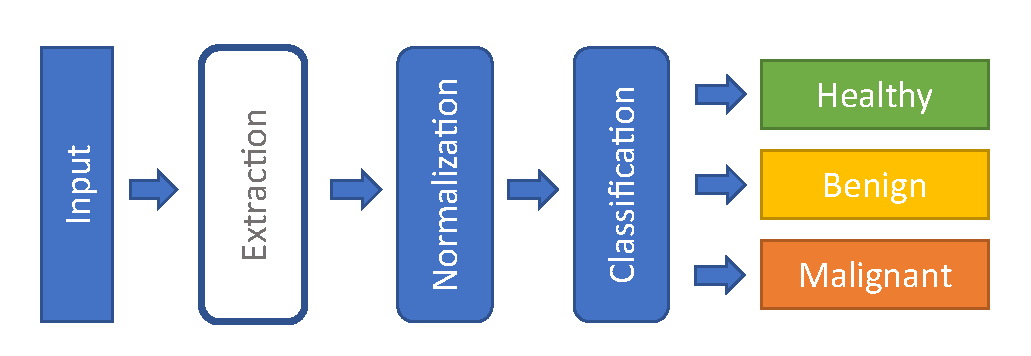
\includegraphics[width=0.8\linewidth]{content/figures/Simple.pdf}
        \legende{Processus de classification.}
        \label{pipeline}
    \end{center} 
\end{figure}
\subsection{Extracteurs de caractéristiques}
La première méthode d'extraction de caractéristiques sur laquelle nous nous appuyons se base sur une décomposition en ondelettes de Daubechies \cite{Halimi2017a}. Cette décomposition est réalisée à quatre échelles différentes. Pour chacune d'elles, nous récupérons un ensemble de coefficients horizontaux, verticaux et diagonaux. Afin de réduire la dimension des descripteurs, la distribution des coefficients est modélisée par une loi normale généralisée centrée dont la densité de probabilité $f$ est décrite par l'\Cref{ggd}, avec $\Gamma$ correspondant à la fonction gamma. Les auteurs de l'étude ne retiennent comme caractéristiques que les paramètres d'échelle $\alpha$ et de forme $\beta$. Dans un but de clarté, nous nommerons cette méthode "Ondelettes" dans les prochains paragraphes. La décomposition par ondelettes est effectuée par la bibliothèque logicielle "PyWavelets" \cite{lee2006pywavelets}.\par
\begin{equation}
    f(x)= \frac{\beta}{2\alpha\Gamma(1/\beta)} e^{-\left(|\frac{x}{\alpha}|\right)^\beta}
    \label{ggd}
\end{equation}
La seconde méthode que nous mettons en oeuvre se base sur treize des caractéristiques définies par Haralick, dont l'efficacité a été démontré sur des images texturées. Ces caractéristiques sont extraites selon les axes horizontal, vertical et les diagonales distinctes. Afin de simplifier la lecture, nous emploierons le terme "Haralick" pour nommer cette méthode dans la suite de cet article. Cette extraction se base sur la bibliothèque logicielle "Mahotas" \cite{coelho2012mahotas}.\par
Enfin, la dernière méthode proposée se base sur les \acs{rnc}, généralement appropriés à la classification d'images. Nous utiliserons à cette fin une architecture de type "InceptionV3" supposée pertinente dans ce cadre d'application \cite{Litjens2017}. Afin de tirer le meilleur parti de cette architecture, nous nous orientons vers de l'apprentissage par transfert. En effet, ce type de techniques est particulièrement adapté à des problématiques suffisamment proche des données initiales, et pour lesquelles la quantité de données disponible est restreinte. Pour cela, nous nous référons à une version de ce modèle entraînée sur la base d'images "ImageNet", dont nous retirons au préalable les couches responsables de la classification. Afin de conserver une cohérence entre le nombre de caractéristiques extraites et le nombre d'échantillons à notre disposition, nous ajoutons également une couche de "Global Pooling" pour réduire la dimension spatiale de chaque carte d'activation à un simple scalaire. Lors de ces prochaines lignes, nous utilisons le terme "\ac{rnc} Max" (respectivement "\ac{rnc} Moy") pour faire référence à un tel réseau comportant respectivement une couche de "Global Pooling" basé sur une fonction de maximum (respectivement moyenne). De plus, nous combinons aux précédents éléments une \ac{pca} afin de réduire considérablement le nombre de variables de manière non supervisée et analyser son incidence. Nous emploierons dans ce cas les termes "\ac{rnc} Max + \ac{pca}" et "\ac{rnc} Moy + \ac{pca}" dans la suite cet article. La manipulation des \ac{rnc} est réalisée grâce à la bibliothèque logicielle "Keras" \cite{chollet2015keras}.\par
La \Cref{variables} synthétise l'ensemble des méthodes d'extraction ainsi que le nombre associé de caractéristiques extraites.
\begin{table}[h]
\centering
    \begin{tabular*}{0.6\linewidth}{l@{\extracolsep{\fill}}l}
        \hline
        \textbf{Méthode} & \textbf{Nombre} \\
        \hline
        Ondelettes & 24 \\
        \hline
        Haralick & 52\\
        \hline
        \ac{rnc} & 2048\\
        \hline
        \ac{rnc}+ \ac{pca} & 20\\
        \hline
    \end{tabular*}
    \caption{Nombre de caractéristiques extraites par méthode.}
    \label{variables}
\end{table}

\section{Données}
\label{donnee}
Les données de cette étude sont fournies par le service de dermatologie de l'hôpital de Saint-Étienne avec consentement du patient et proviennent d'une base contenant trois types d’images : Photographie clinique, Dermatoscopie et \ac{mcr}. De plus, chaque patient est associé à une vérité terrain tirée de l’histopathologie \cite{Cinotti2018}.\par
Les images de la modalité \ac{mcr} sont acquises au niveau de la jonction dermo-épidermique jugée pertinente pour le diagnostic du Lentigo bénin et malin par le spécialiste. Ces images natives peuvent contenir différents types de tissus, lésionnel ou non, et ont une résolution spatiale de 1000 pixels par 1000 pixels, avec une quantification sur un seul canal de 8 bits.\par
Un premier jeu de données est constitué à partir de la base d'images initiale et avec l’aide du spécialiste. Des annotations sont réalisées sur 68 patients, soit 2089 images \ac{mcr}, selon trois critères : "Malin" pour les images comprenant au moins du tissu malin, "Bénin" pour les images composées d'une pathologie bénigne et enfin une étiquette "Sain" correspondant à l'absence de ces deux caractéristiques. Les ratios associés à ce jeu de données sont les suivants: 38\% de données Maligne, 37\% de données Saines et 25\% de données Bénigne. Nous nommerons ce jeu de données "Images Originales".\par
Un second jeu de données dérivé des images natives est également constitué, afin d'évaluer la capacité à différencier les types de tissus. A cette fin, une interface graphique permettant de réaliser des sous-images de 250 pixels par 250 pixels est mise à disposition du spécialiste. Ainsi, 200 sous-images incluant un type de tissu particulier sont extraites pour chacune des trois annotations mentionnées précédemment. Des exemples de ces sous-images extraites par le spécialiste sont visibles en \Cref{donnees}. Nous nommerons ce jeu de données "Sous-images".\par
\begin{figure}[h]
    \begin{center} 
        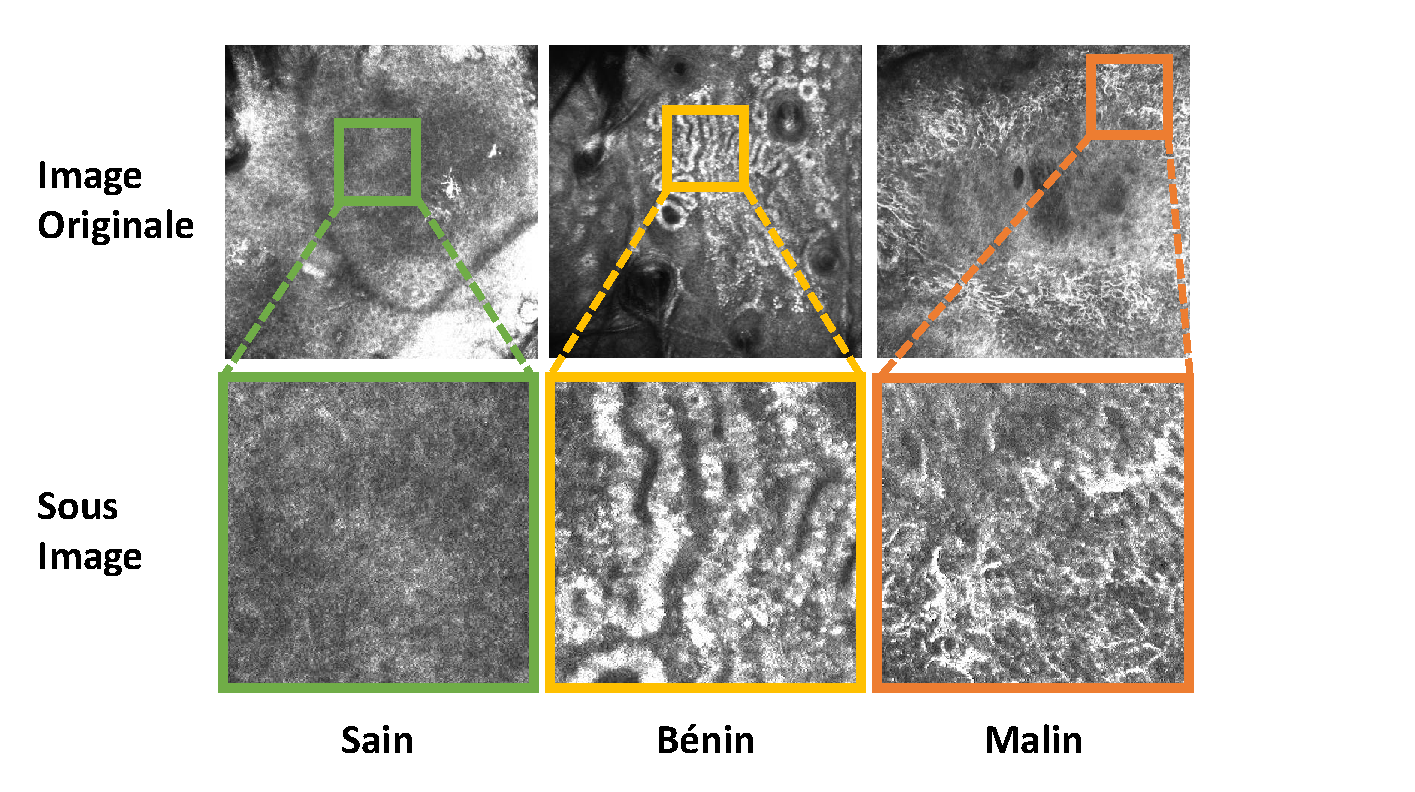
\includegraphics[width=0.9\linewidth]{content/figures/Donnees.pdf}
        \legende{Exemple de données originales et de sous-images extraites par le spécialiste.}
        \label{donnees}
    \end{center} 
\end{figure}
\section{Résultats}
\label{resultat}
Le protocole de validation employé est équivalent lors de chaque expérience. Pour ce faire, nous réalisons une validation croisée imbriquée afin de permettre une sélection des hyperparamètres du modèle \ac{svm}, tout en assurant son évaluation objective \cite{Cawley2010}. Chacune des étapes de validation croisée est basée sur une stratégie de type "K-Fold" sur 5 échantillons. Nous utilisons la bibliothèque "Scikit Learn" pour réaliser ces démarches de validation, ainsi que pour la classification et l’évaluation des mesures \cite{pedregosa2011scikit}.\par
Chaque expérience est évaluée à l'aide du F1-Score, dont la valeur tend vers 1 conjointement à la Précision et au Rappel, et permet une meilleure objectivité dans une situation où les données sont non balancées. De plus, un écart-type est calculé afin d'analyser la stabilité des modèles lors de la validation croisée imbriquée.\par
La \Cref{scores} met en avant les différents F1-Scores obtenus lors de l'évaluation de chaque expérience, selon leur évaluation sur le jeu de données utilisant les images originales ou les sous-images.\par
Tout d'abord, nous remarquons une stabilité accrue de l'ensemble des méthodes évaluées et ce quel que soit l'échantillon utilisé lors de l'évaluation.\par
En revanche, nous obtenons des résultats mitigés lors de l'évaluation sur les images originales. La méthode basée sur la décomposition par ondelette semble peu concluante dans ces conditions. Nous retrouvons des performances acceptables avec l'extraction des caractéristiques d'Haralick ainsi qu'avec les "\ac{rnc} Max", "\ac{rnc} Max\-+\ac{pca}" et "\ac{rnc} Moy+\ac{pca}". Par ailleurs, nous émettons une réserve concernant l'extraction "\ac{rnc} Moy", et ce malgré le dispositif de validation mis en place, dans la mesure ou le nombre de caractéristiques extraites avoisine le nombre d'observations à disposition.\par
Afin de vérifier la pertinence de ces méthodes à discriminer les différentes formes de tissu, nous avons réalisé leur évaluation sur la base de sous-images. Nous pouvons observer de très bons résultats sur l'ensemble des méthodes dans ces conditions d'évaluation. Cette fois-ci, la méthode basée sur la décomposition par ondelettes semble plus apte à caractériser ces sous-images que les descripteurs d'Haralick. En revanche, les méthodes basée sur \ac{rnc} semblent exceller à cette tâche de classification. Néanmoins, nous devons émettre une réserve sur les résultats concernant le "\ac{rnc} Max" et "\ac{rnc} Moy" et ce malgré le processus de validation mis en place. En effet, le nombre de caractéristiques extraites est nettement supérieur au nombre d'observations (600 observations pour 2048 variables) pouvant conduire à des résultats trop optimistes.\par

\begin{table}[h]
\centering
    \begin{tabular*}{\linewidth}{l@{\extracolsep{\fill}}ll}
        \hline
        \textbf{Méthodes} & \textbf{Images Originales} & \textbf{Sous-images}\\
        \hline
        Ondelettes & 0.62$\pm$0.01 & 0.87$\pm$0.02\\
        \hline
        Haralick & 0.71$\pm$0.02 & 0.82$\pm$0.01\\
        \hline
        \ac{rnc} Max & 0.76$\pm$0.02 & 0.97$\pm$0.02\\
        \hline
        \ac{rnc} Max + \ac{pca} & 0.75$\pm$0.01 & 0.95$\pm$0.02\\
        \hline
        \ac{rnc} Moy & 0.86$\pm$0.02 &0.99$\pm$0.01\\
        \hline
       \ac{rnc} Moy + \ac{pca} & 0.76$\pm$0.01 & 0.95$\pm$0.01\\
    \end{tabular*}
    \caption{Performances mesurées sur diverses méthodes à l'aide du F1-Score.}
    \label{scores}
\end{table}

\section{Conclusion et Perspectives}
\label{conclusion}
Dans cette étude nous avons évalué la pertinence de trois extracteurs de caractéristiques dans le cadre d'images \ac{mcr}. Ces diverses méthodes, et plus particulièrement les \ac{rnc} nous permettent de réaliser une classification robuste sur des sous-images dont la pathologie est isolée. Celle-ci est en revanche plus complexe sur les images originales et ce quelque soit la méthode utilisée.\par 
L'une de nos hypothèses non formulée supposait une supériorité lors de la classification de la couche de "Global Pooling" basée sur une fonction de type moyenne par rapport à une fonction de type maximum. Cette hypothèse se fondait sur une plus grande tolérance au bruit de la moyenne. Or dans ce cadre, notre travail suggère une faible influence de ce paramètre sur les résultats.\par
De futures investigations devraient permettre une meilleure classification de ces images. La première piste envisagée se base sur un découpage de l'image \ac{mcr} et sur l'agrégation de caractéristiques à basse échelle. La seconde approche centrée sur les \acs{rnc}, consistera à analyser l'impact du "fine-tuning" sur la capacité du modèle à classifier ces même images. De plus nous souhaiterions par cette approche exploiter le potentiel des cartes d'activations générées par ces réseaux pour réaliser des segmentations par apprentissage faiblement supervisé.\par
Ce travail s'inscrit comme le premier maillon d'un ensemble de travaux et devrait, à plus long terme, nous permettre d'envisager une prise de décision au niveau du patient, voire également multi-modale par l'utilisation des autres modalités d'image.\par

\section*{Remerciements}
Ces travaux ont été réalisés dans le cadre d'un financement proposé par le Conseil Régional de Bourgogne Franche Comté et d'un co-financement par le Fonds européen de développement régional.\par
Nous tenons à remercier le Dr. Perrot ainsi que le Dr. Cinotti pour leur mise à disposition de la base d'images, mais également pour leur précieux travail d'annotation.

% {\small
% \printbibliography
% }

\bibliography{content/bibliography.bib}
\end{sloppypar}
\end{document}